\documentclass[10pt,a4paper]{article}
\usepackage[margin=20mm]{geometry}
\usepackage[T1]{fontenc}
\usepackage[utf8]{inputenc}
\usepackage{lmodern,microtype,amsmath,amssymb,booktabs,graphicx,xcolor}
\usepackage[hidelinks]{hyperref}
\setlength{\parindent}{0pt}\setlength{\parskip}{4pt}
\title{On the possibility of an analytic expression for the extremal mass\\
\large of equal-spin rotating black holes in five-dimensional Einstein--Gauss--Bonnet gravity}
\author{Review by Claude (Fable 5.1), for C.~Bejarano}
\date{27 October 2026}
\begin{document}
\maketitle
% Body of the English report on the analytic expression. Included by review-report.tex and by
% analytic-expression-report.tex (standalone).

\subsection*{Question}

Is there an analytic expression for the extremal mass $M_{\rm ext}(J,\alpha)$ of the
five-dimensional, asymptotically flat, equal-spin ($J_1=J_2=J$) Einstein--Gauss--Bonnet black
hole, action $(16\pi G_5)^{-1}\!\int\!\sqrt{-g}\,(R+\alpha\mathcal L_{\rm GB})$, $G_5=1$?
Scale invariance reduces the problem to one function of one variable,
\begin{equation}
 M_{\rm ext}=\pi^{1/3}J^{2/3}\,m(s),\qquad s=\frac{\pi^{2/3}\alpha}{J^{2/3}},
 \qquad\text{equivalently}\qquad \mu(y)=\frac{M_{\rm ext}}{J^{2/3}}=\pi^{1/3}m(\pi^{2/3}y),\ \ y=\frac{\alpha}{J^{2/3}},
\end{equation}
and the slope studied in the manuscript is $\partial M_{\rm ext}/\partial\alpha|_J=\mu'(y)=\pi\,m'(s)$.

\subsection*{Short answer}

A closed form for $m(s)$ is not available and, on the present evidence, is not feasible with
the tools used in this project. What \emph{is} established, and what this review verified
independently, is an exact description of both ends of the function and of the near-horizon
data at every coupling, together with a global representation accurate to $10^{-5}$. No new
closed form was found here; one further natural attempt (expansion in the algebraic throat
variable) was made and is reported below as a negative result.

\subsection*{What is known exactly}

\paragraph{Weak coupling.} The project's exact exterior solver (\texttt{extremal-mass/code/pert.py})
gives, with $\zeta_n=\zeta(n)$,
\begin{align}
 m(s)&=\tfrac32+s-\tfrac{236}{105}s^2+d_3s^3+d_4s^4+d_5s^5+d_6s^6+\dots,\\
 d_3&=\tfrac{60851752}{33075}-1536\,\zeta_3=-6.548307\ldots,\qquad
 d_4=-\tfrac{592541765354296}{1489863375}+\tfrac{227328}{5}\zeta_3+\tfrac{88064}{25}\pi^4=66.100522\ldots,\nonumber\\
 d_5&=\tfrac{447853140007115845664}{6100990520625}+\tfrac{657983488}{175}\zeta_3-\tfrac{3972366336}{625}\zeta_2^2-\tfrac{1464139776}{25}\zeta_5\nonumber\\&=423.920197\ldots,\nonumber\\
 d_6&=-4737.494827\ldots\ \ (\text{exact form in \texttt{extremal-mass/series/coefficients.json}}).\nonumber
\end{align}
The first two terms are the published result of Ma, Li and L\"u. The coefficients are exact
conditional on the identification (PSLQ at 100 digits) of regularised horizon constants with
multiple zeta values; the audit found that this identification is over-determined by the
horizon-regularity conditions of the solver (injecting a wrong value for one constant makes the
order-3 run abort with ``$h$ not regular''), and the rational horizon shifts $X_5,X_6$ coincide with
an independent algebraic prediction. The series is therefore trustworthy. Its radius of
convergence is small: the throat data have a square-root branch point at
$s_*=0.00592\pm0.05482\,i$, $|s_*|=0.0551$; the six known $d_n$ are compatible with, but do not
establish, the same radius for $m(s)$ (the ratio test on six terms only bounds it by roughly
$0.12$).

\paragraph{Near-horizon data at any coupling.} Writing $g_H=r_H^2$, $a=\alpha/g_H$ and
$q=h_H/g_H$ for the horizon squashing, Sen's entropy function on the throat
$\mathrm{AdS}_2\ltimes S^3$ gives (rederived here from scratch, 12 assertions in
\texttt{checks/check\_throat2.py})
\begin{gather}
 16a^2q^2(4-q)-8a(2q^2-7q+4)+q-2=0,\qquad
 \frac{8J^2}{\pi^2g_H^3}=\frac{q^2(4-q)\,[1+4a(4-3q)]}{8},\label{eq:throat}\\
 S_{\rm ext}=\frac{\pi^2}{2}\,g_H^{3/2}\sqrt q\,\bigl[1+4a(4-q)\bigr],\nonumber\\
 v_1=\frac{(1+4aq)(12aq-16a-1)}{4(6aq^2-16aq-1)},\qquad
 e^2=\frac{(q-4)(1+4aq)^2(12aq-16a-1)}{4q\,(6aq^2-16aq-1)^2},\nonumber
\end{gather}
with $v_1$ the $\mathrm{AdS}_2$ radius squared and $e$ the fibre electric field. At fixed $J$
these equations determine $g_H(s)$, $q(s)$ and $S_{\rm ext}(s)$ as algebraic functions. They do
\emph{not} determine the mass: $M_{\rm ext}$ needs the asymptotic normalisation of the time
coordinate, which the throat discards. (Equation (3.18) of Kleihaus--Kunz--Radu prints the total
$J_1+J_2$; the project's per-plane normalisation is the consistent one.)

\paragraph{Strong coupling.} Matched asymptotics and, independently, a BTZ dictionary for the
small-$r$ core of static EGB black holes give
\begin{equation}
 m(s)=\frac{3s}{4}+\frac43\,s^{-1/2}+a_2\,s^{-1}+a_3\,s^{-3/2}+\dots,\qquad
 M_{\rm ext}=\frac{3\pi\alpha}{4}+\frac{4J}{3\sqrt\alpha}+a_2\frac{J^{4/3}}{\pi^{1/3}\alpha}+\dots
\end{equation}
The leading term is the mass of the nakedly singular static solution (the endpoint conjectured
by Kleihaus, Kunz and Radu); $a_1=4/3$ is derived under the assumption that the rotating
extremal core obeys the static BTZ dictionary and is confirmed numerically to $4\times10^{-4}$;
$a_2=0.456527$ is a conditional analytic value, numerically $0.4566\pm0.0002$; $a_3\simeq-0.263$
is purely numerical. The audit noted that the BTZ relation, taken literally beyond leading
order, would give $a_2=0$, so the dictionary is a leading-order statement only.

\paragraph{Exact identities that constrain any candidate.} The Smarr relation at $T=0$ gives
$M_{\rm ext}=3\Omega_HJ+\alpha\,\partial M_{\rm ext}/\partial\alpha|_J$, i.e.
$3\,\Omega_HJ^{1/3}=\mu-y\mu'$, so the minimum of the slope is the maximum of the scaled horizon
angular velocity; the first law at $T=0$ gives $\partial M_{\rm ext}/\partial J|_\alpha=2\Omega_H$.
Both hold on all three numerical branches checked here.

\subsection*{Numerical knowledge, cross-validated}

Three independent determinations exist in the repository: the manuscript's zero-temperature
extrapolation of non-extremal solutions (13 couplings, $s\le1.10$), the direct $T=0$ spectral
solver of \texttt{work/kkr-extremal} ($s\le5.2$), and the shooting / multiple-shooting branch
of \texttt{extremal-mass/strong} ($2\le s\le103$). This review compared them with each other,
with the exact series and with the ten-term global approximant (table~\ref{tab:threeroutes},
figures~\ref{fig:three}--\ref{fig:slope}): $m$ agrees to $6\times10^{-6}$ relative across all
sources, the slope to $3\times10^{-4}$ (within the manuscript's own fit envelopes), and the
minimum of the slope is $\partial M_{\rm ext}/\partial\alpha|_J\simeq1.070$ at
$y\simeq0.19$ ($s\simeq0.40$) on every route. The approximant
\begin{equation}
 m(s)\simeq\frac{3s}{4}+\sum_{k=1}^{10}c_k\,t^k,\qquad t=\Bigl(1+\frac s\kappa\Bigr)^{-1/2},\quad
 \kappa=0.356242695,
 \label{eq:approx}
\end{equation}
with
\begin{equation*}
\begin{aligned}
 c_{1\ldots5}&=2.233910,\ 1.281505,\ -0.713812,\ 6.055449,\ -75.189708,\\
 c_{6\ldots10}&=230.148117,\ -352.252482,\ 303.906361,\ -142.214324,\ 28.244984,
\end{aligned}
\end{equation*}
reproduces $m(0)=3/2$, $m'(0)=1$,
$a_1=4/3$, $a_2=0.456527$ exactly and every numerical point to $1.1\times10^{-5}$. It is the
best available ``expression'' for practical use, but it is an interpolant: its Taylor
coefficients beyond $s^1$ and its $s^{-3/2}$ coefficient ($-0.15$ instead of $-0.26$) are not
those of $m(s)$.

\subsection*{Why a closed form is unlikely, and what was tried}

\begin{enumerate}
\item \textbf{Transcendental structure.} $d_n$ contains multiple zeta values of weight up to $n$
 ($\zeta_3$ at order 3, $\zeta_2^2$ at order 4, $\zeta_5$ at order 5, $\zeta_3^2$ and
 $\zeta_2^3$ at order 6). An algebraic function of $s$ over $\mathbb Q$, or a hypergeometric-type
 function of $s$ with rational parameters, has rational Taylor coefficients. Zeta values of
 growing weight arise instead when the \emph{parameters} of such functions depend on $s$,
 for instance through $\Gamma$-functions of the throat exponent $\gamma(s)$, which is exact
 and irrational ($\lambda^2+\lambda=Q(a,q)$ in the project's endpoint report). Any closed form
 would therefore have to be non-elementary, with $s$ entering through exponents.
\item \textbf{Singularities.} The weak series has complex singularities close to the origin
 (conjecturally $s_*$, radius $0.055$); the function has an essential change of behaviour at
 $s\to\infty$ (expansion in $s^{-1/2}$ after a linear term). A simple formula interpolating the
 two ends and respecting $s_*$ was sought by the previous session without success
 (finite-Laurent Hamilton--Jacobi superpotentials, Liouvillian solutions of the squashing
 equation --- its Galois group is $SL(2,\mathbb C)$ --- and a resonant candidate ODE for $m(s)$,
 all ruled out).
\item \textbf{New attempt in this review: the throat variable.} Since $s_*$ is a critical
 point of the exact algebraic map $s(q)$, the fold disappears in the variable $q$; both ends of
 the branch are series in $q$ ($q\to2$ at Myers--Perry, $q\to0$ at strong coupling, with
 $s^{-1/2}\propto q$ there). We composed the exact series with $s(q)$ and expanded
 $y(q)=m-3s/4$ in $w=2-q$:
 $y=\tfrac32+0.03125\,w-0.05595\,w^2+0.10348\,w^3-0.26867\,w^4+0.65415\,w^5-1.80098\,w^6+\dots$
 The coefficients grow geometrically with ratio $\approx-2.6$, i.e.\ radius $|w|\approx0.4$, and
 the exact discriminant $D(q)=5q^4-34q^3+73q^2-56q+16$ of the throat vanishes at $q=2.2763$,
 $|2-q|=0.276$: on the branch continued to negative coupling $q$ has an extremum there, so $q$
 is not a uniformising coordinate near Myers--Perry. Against the numerics the $w$-series is
 \emph{worse} than the $s$-series (error $2.6\times10^{-3}$ at $s=0.044$ versus
 $7.5\times10^{-6}$), and a $[3/3]$ Pad\'e in $w$ fails beyond $s\approx0.05$. A $[3/3]$ Pad\'e
 of $m(s)$ itself extends the useful range only to $s\approx0.4$ (error $5\times10^{-3}$) and
 is useless beyond $s\approx0.7$. Negative result; receipts in
 \texttt{checks/receipts/uniformize\_q.txt}.
\end{enumerate}

\subsection*{What would move the question}

(i) An exact derivation of $a_2$ from the next order of the core/intermediate matching, which
would fix the strong-coupling side to two exact terms; (ii) one or two more exact orders
$d_7,d_8$ (the solver scales badly: order 6 took 1\,h\,38\,min and 200\,MB) to test the
conjectured radius $|s_*|$ and the large-order form $d_n\sim2\,\mathrm{Re}[C\,s_*^{-n}n^{\beta}]$;
(iii) a search for a resummed structure in which $s$ enters through the exact throat exponent
$\gamma(s)$, e.g.\ ratios of $\Gamma$-functions reproducing the weight pattern of the $d_n$;
(iv) a proof, from the horizon expansion in $r^{2\gamma}$, that $m(s)$ inherits the throat fold.
None of these is a small task, and none is guaranteed to yield a closed form. Until then the
honest statement is: $M_{\rm ext}(J,\alpha)$ is known exactly as two asymptotic expansions, its
near-horizon data are algebraic at every coupling, and the function in between is known
numerically to $10^{-5}$ and summarised by eq.~\eqref{eq:approx}.


\begin{table}[h]
\centering\footnotesize
\begin{tabular}{@{}p{.5\textwidth}cp{.33\textwidth}@{}}
\toprule
comparison (worst over the common range) & quantity & deviation\\
\midrule
manuscript $T\to0$ vs exact weak series ($s<0.055$) & $m$ & $4.9\times10^{-6}$ rel.\\
manuscript $T\to0$ vs global approximant (13 rows) & $m$ & $6.4\times10^{-6}$ rel.\\
manuscript $T\to0$ vs direct $T=0$ solver & $\mu$ & $2.4\times10^{-5}$\\
manuscript $\Psi_{\rm ext}$ vs $\pi m'$ of the approximant & slope & $2.1\times10^{-3}$\\
manuscript $\Psi_{\rm ext}$ vs direct $T=0$ solver $\mu'$ & slope & $3.0\times10^{-4}$\\
multiple-shooting table ($2\le s\le103$) vs approximant & $m$ & $6.9\times10^{-6}$ rel.\\
\midrule
minimum of the slope: approximant / direct solver / manuscript lowest sample & $\mu'$ & $1.0700\,(y{=}0.185)$ / $1.0698\,(y{=}0.195)$ / $1.0715\,(y{=}0.175)$\\
\bottomrule
\end{tabular}
\caption{Cross-validation of the three independent numerical determinations
(\texttt{checks/check\_branch\_consistency.py}).}
\label{tab:threeroutes}
\end{table}

\begin{figure}[h]\centering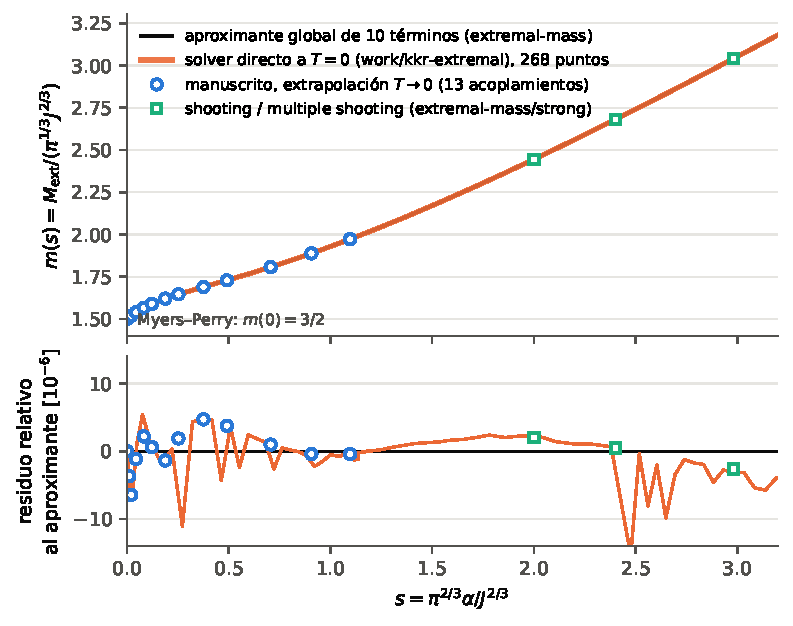
\includegraphics[width=.8\textwidth]{figures/fig-three-routes.pdf}
\caption{The three numerical routes and the global approximant; lower panel: relative residuals.}\label{fig:three}\end{figure}
\begin{figure}[h]\centering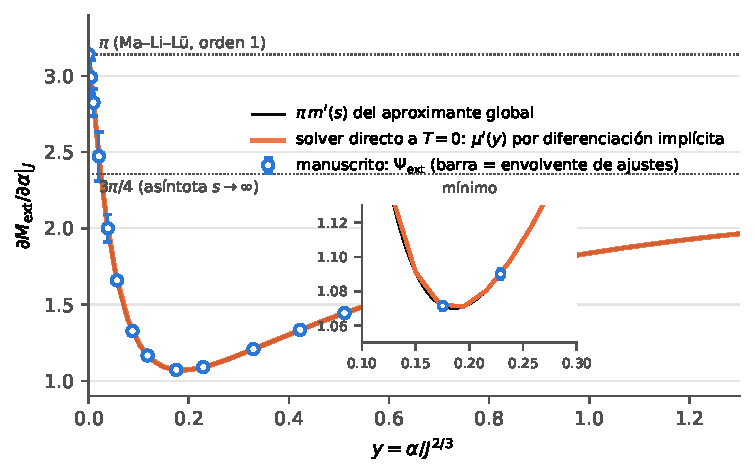
\includegraphics[width=.8\textwidth]{figures/fig-slope.pdf}
\caption{The slope $\partial M_{\rm ext}/\partial\alpha|_J$ by the three routes.}\label{fig:slope}\end{figure}
\end{document}
